\documentclass[12pt]{article}
\usepackage[left=2cm, top=2cm, right=2cm, bottom=2cm]{geometry}
\usepackage[utf8]{inputenc}      % accents dans le source
\usepackage[T1]{fontenc}
\usepackage[french]{babel}
\usepackage{graphicx}
\usepackage{graphics}
\usepackage{amsmath}
\usepackage{tikz}
\usepackage{xcolor} 
\usepackage{mathtools}
\usepackage{parskip}
\usepackage{subcaption}
\usepackage[export]{adjustbox}

\title{\vspace{-2cm}\textbf{TP 2 - Ondes progressives ultrasonores}}
\author{\vspace{-0.5cm}MENARD Alexandre - VIEILLEDENT Florent}
% \setlength{\parindent}{1cm}
\date{\vspace{-0.7cm}}

\begin{document}
\maketitle

L'acoustique est l'étude des ondes sonores dans différents milieux. Elle trouve des applications dans le développement des chambres
anéchoïques où l'on cherche à minimiser au maximum les perturbations sonores pour permettre des mesures précises sur le son émis par des appareils par exemple. 
Notre travail ici consistera à caractériser les ondes sonores progressives ultrasonores par observation qualitative. Nous proposerons
deux protocoles pour déterminer la célérité de ces dernières et nous mesurerons les coefficients de transmission et réflexion pour différents matériaux.

\section{Mesure de la célérité du son}
Dans cette partie, nous mesurerons la célérité du son à l'aide de la longueur d'onde et de la fréquence du son émis mais aussi par une seconde méthode basée sur la réflexion de l'onde.

\subsection{Génération et caractérisation d'une onde sonore}
L'émetteur sonore est composé d'un matériau dit piézo-électrique capable de se déformer sous un champ électrique. Ainsi, soumis à un champ électrique
le matériau va se déformer et générer un déplacement du milieu donc une onde sonore. Pour une première approche, nous suivons le protocole
expérimental dans la section \textbf{1.1}. Nous observons alors pour l'émetteur que le signal est émis en continu puis ensuite n'est plus émis sous la forme d'un signal en créneau avec une amplitude de $13V$.
Le signal reçu est sinusoïdal avec une amplitude constante de l'ordre de $500mV$\footnote{La valeur dépend de la distance émetteur-récepteur, nous avons relevé un maxima à 1.5V à une distance presque nulle, mais nous discuterons de cette caractéristique dans la dernière partie.}. De plus, nous relevons bien une fréquence conservée entre l'émetteur et le récepteur. Plus le récepteur est éloigné de l'émetteur, plus l'amplitude mesurée est faible, mais la fréquence n'est pas modifiée.

Nous passons ensuite l'émetteur en mode "salves courtes" dans la même configuration qu'avant. Nous observons alors des signaux de la forme suivante:
\begin{figure}[!htbp]
	\centering
	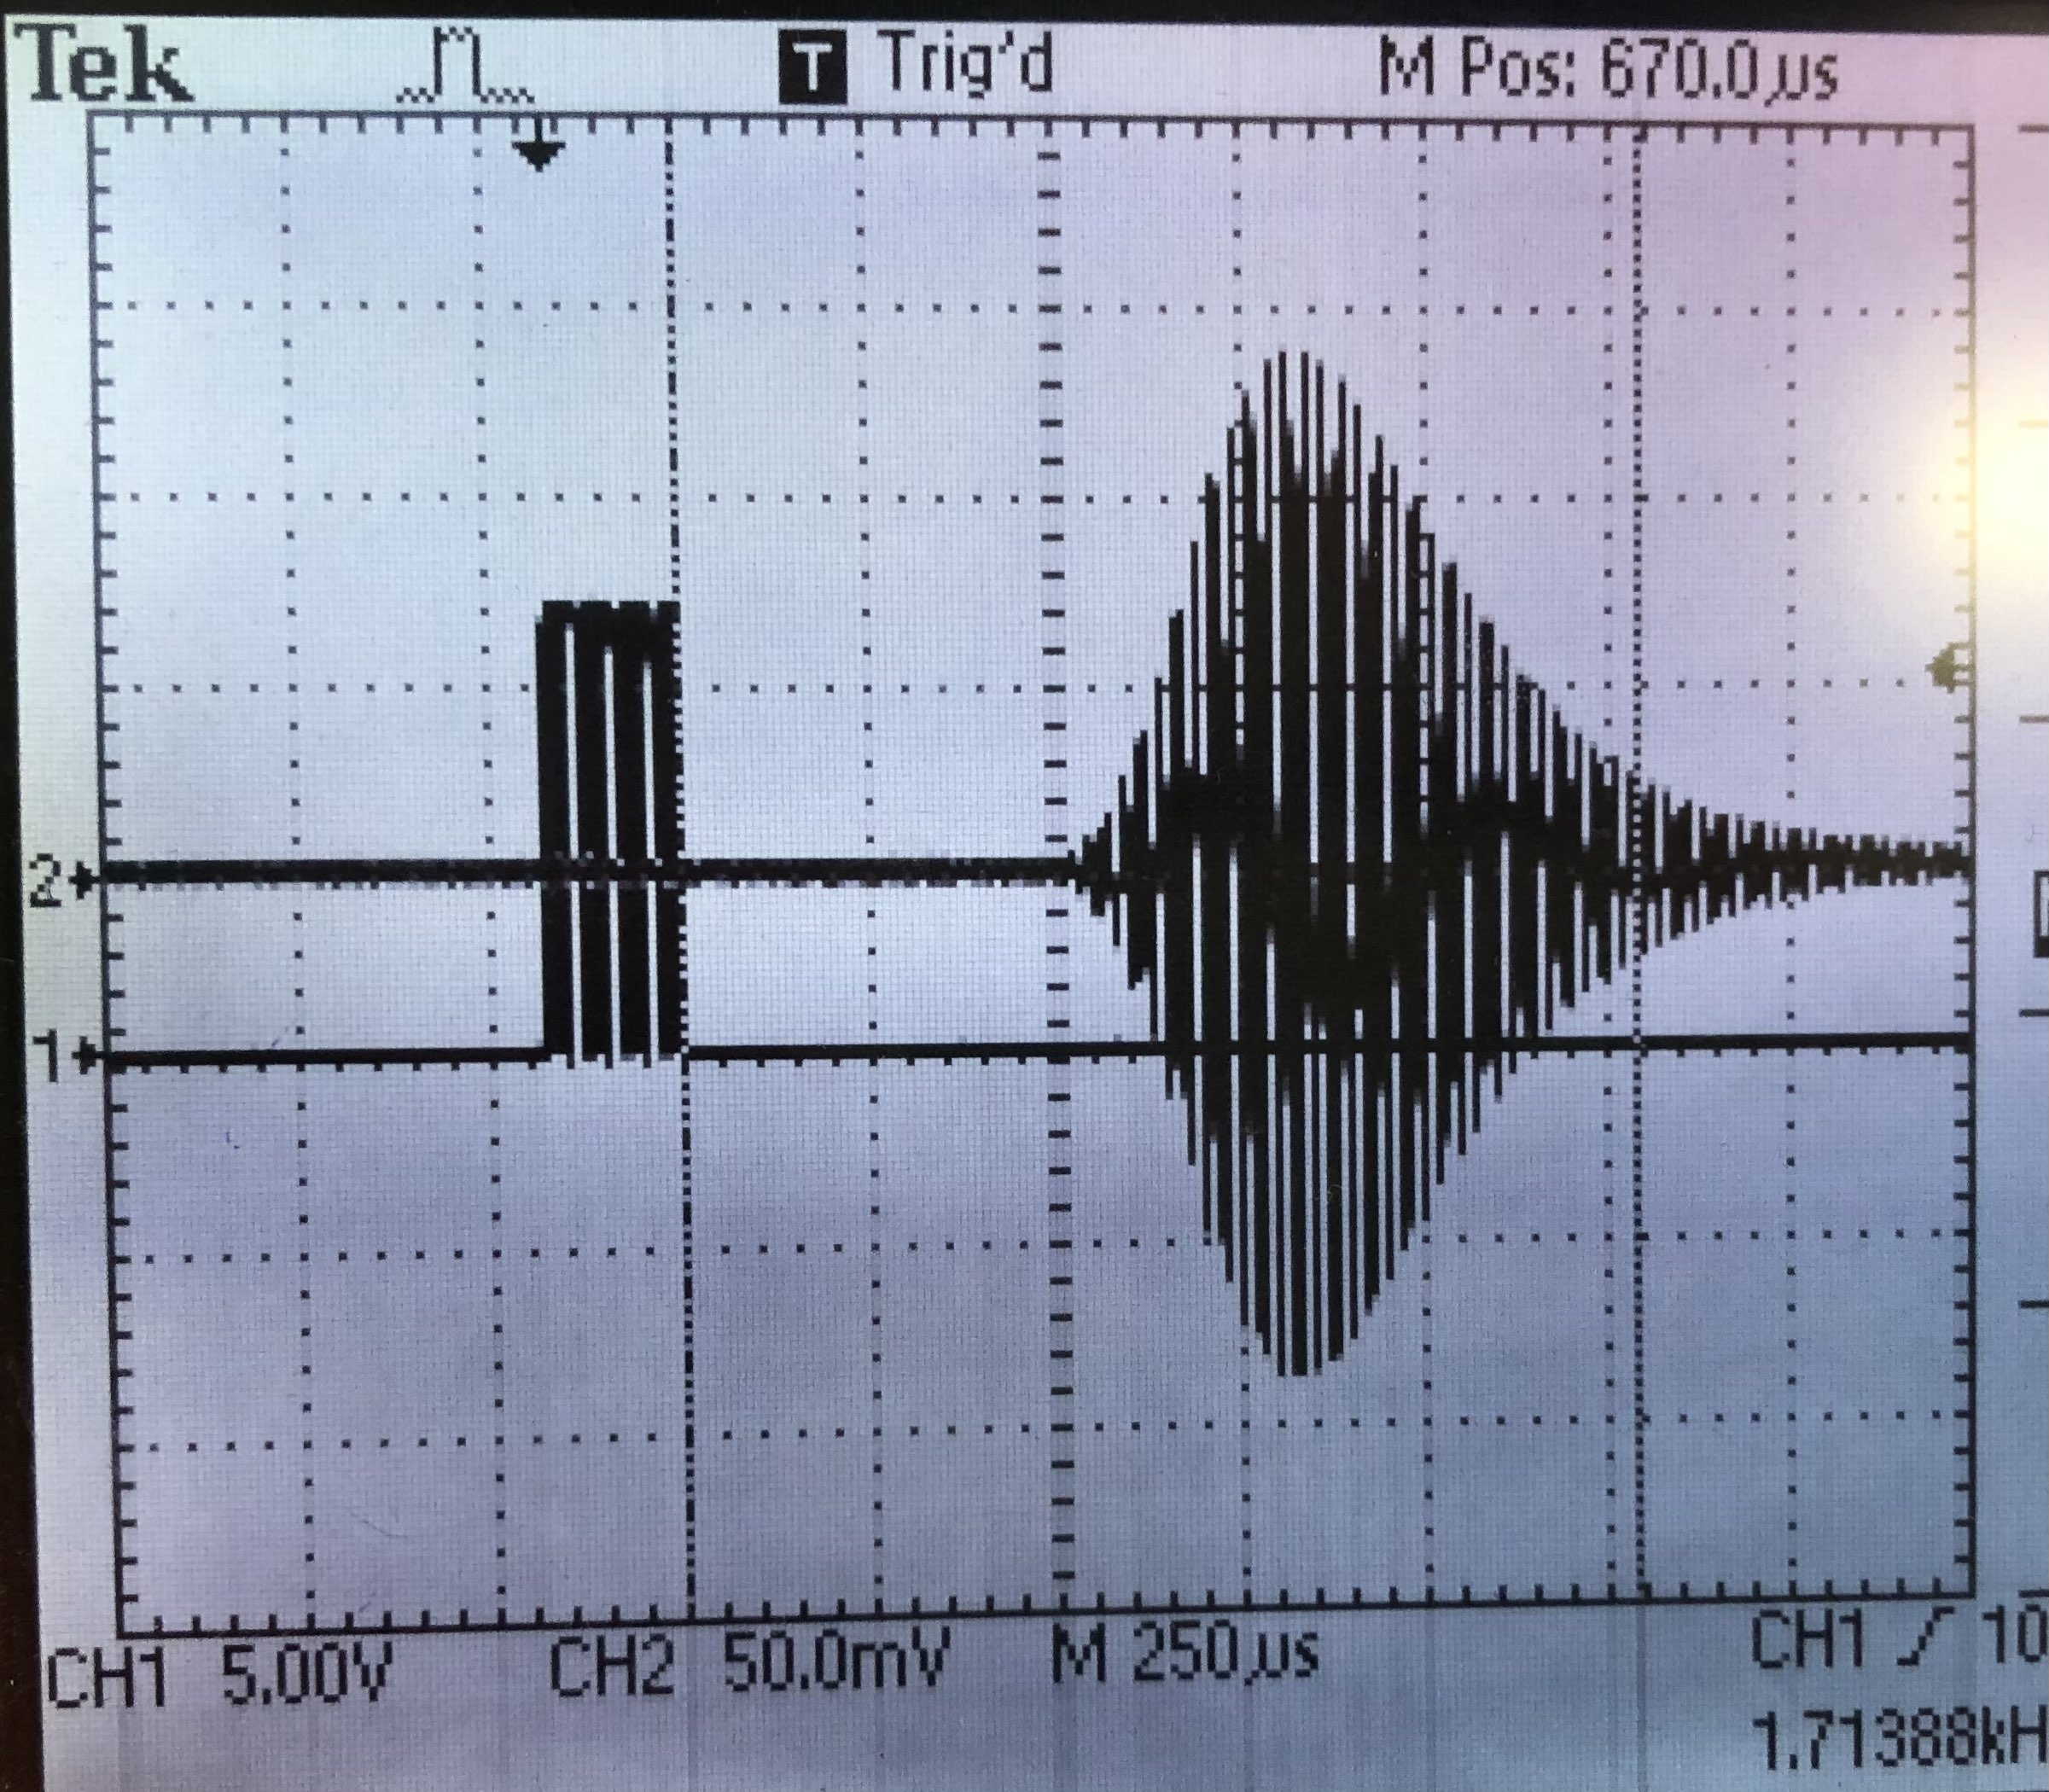
\includegraphics[width=0.25\textwidth]{img/salves_courtes.jpg}
	\hfill
	\caption{Signal émis en salves courtes}
\end{figure}

On remarque le même signal en créneau de l'émetteur, ainsi qu'un signal sinusoïdal reçu qui augmente en amplitude jusqu'à un maximum puis redescend rapidement à une amplitude nulle. L'écart étant dû à la distance entre l'émetteur et le récepteur.

\subsection{Modèle}
En suppose que l'onde émise est parfaitement sinusoïdale, nous pouvons modéliser la propagation de cette dernière avec $k=\frac{2\pi}{\lambda}$, $\nu$ la fréquence, $\phi$ la phase à l'origine et $A(x)$, l'amplitude selon $x$:
\begin{align}
	y(x, t) = A(x) \sin(2\pi\nu t - kx + \phi)
\end{align}

Si deux signaux (émis ou reçus) sont en phase, on a alors en deux positions $x_1$ et $x_2$:
\begin{align*}
	y(x_1, t) = y(x_2, t) & \Rightarrow |x_1 - x_2| = n\lambda
\end{align*}

La célérité de l'onde sera alors donnée par $c = \lambda \nu$. Dans le cas d'une mesure par réflexion, si l'on note $\Delta t$ le temps de trajet de l'onde, et $d$ la distance parcourue, on aura $c = \frac{d}{\Delta t}$

\subsection{Protocole expérimental}
Nous suivrons les protocoles expérimentaux 1 et 2 fournis dans la section \textbf{1.2} pour relever une vingtaine de positions dont 10 avec un seul récepteur en mouvement devant être en phase avec le signal émetteur, et 10 autres
avec un récepteur fixe et un second en mouvement où les deux signaux reçus doivent être en phase. L'intérêt de relever une vingtaine de mesures de $\lambda$ permettra de déterminer une incertitude associée statistiquement mais aussi de la réduire le plus possible. A l'aide des curseurs que l'on positionne de façon la plus large puis la plus serrée possible, nous obtenons deux bornes de la fréquence.
On obtient alors par la moyenne $\nu = 37.9 \pm 0.9 kHz$. Les positions des récépteurs et de l'émetteur sont notés $x_{re_1}, x_{re_2}, x_{em}$ et ont des incertitudes associées
$\delta x = 0.2cm$ que l'on détermine par les graduations fournies par le rail gradué mais aussi par l'incertitude sur la position exacte de la surface qui reçoit l'onde. 
Nous utilisons le mode \textit{trigger} de l'oscilloscope pour mettre en arrêt le balayage lorsque le signal dépasse un seuil pour observer un signal fixe.
\begin{figure}[!htbp]
	\centering
	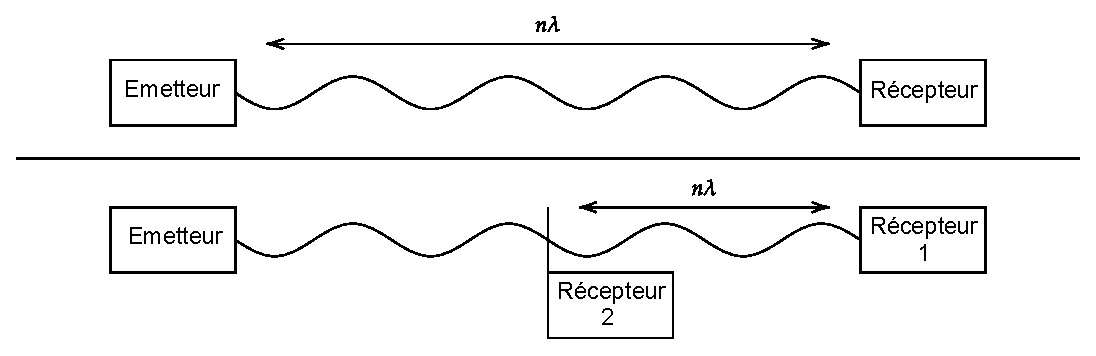
\includegraphics[width=0.6\textwidth]{img/schema}
	\hfill
	\caption{Schéma des deux protocoles 1 et 2}
\end{figure}

Nous proposons également d'effectuer une mesure de la célérité par réflexion en plaçant un écran réflechissant à une distance $d$ de l'émetteur, et en positionnant le récepteur à côté de l'émetteur pour capter l'onde réflechie.
L'écart $e$ entre l'émetteur et le récepteur étant très petit devant la distance $d$, on peut donc négliger l'écart entre le trajet réel et le trajet approché car largement plus faible devant l'incertitude due à nos mesures.\footnote{On note une erreur de l'ordre de 0.4 pour $d > 30cm$, voire Annexe pour démonstration.}

Enfin, nous mesurons la température de la pièce $\theta = 20 \pm 3 \text{°} C$ pour comparer au modèle théorique.

\subsection{Résultats expérimentaux et conclusion}
Dans cette partie, l'ensemble des incertitudes découle de la méthode de propagation des incertitudes d'additions/quotients/produits.
Pour la mesure de la longueur d'onde, nous obtenons $\lambda = 9.3 \pm 0.3 \mu m$, ce qui donne finalement une mesure de la célérité $c = 352 \pm 13 m/s$. Les mesures par réflexion nous donne $c = 325 \pm 8 m/s$. 
Quant à la formule fournie, elle donne une valeur de $c = 343.6 \pm 1.8 m/s$.

Nous remarquons que la mesure par longueur d'onde est cohérente avec la valeur théorique qui rentre dans les bornes de nos incertitudes. Cependant, la mesure par réflexion
n'est pas en accord avec la mesure faite par les longueurs d'ondes. Cet écart est explicable par des conditions expérimentales qui ont changé entre les deux expériences, les fenêtres étant ouvertes à côté
de notre banc de mesure, pouvant faire nettement chuter la température entre les deux mesures. Cependant, il serait pertinent de réaliser des mesures sur des distances $d$ plus grandes avec un émetteur plus puissant
pour réaliser un plus grand nombre de mesures dans des conditions stables, et pourrait permettre de réduire les incertitudes sur notre valeur.


\section{Réflexion et transmission}
\subsection{Modèle}
On définit le coefficient de transmission d'un matériau comme le rapport entre l'amplitude de l'onde transmise par le matériau et l'amplitude incidente, le tout élevé au carré. Le coefficient de réflexion est définie  de la même manière en remplaçant l'onde transmise par l'onde incidente. On néglige pour l'instant l'absorption des ondes.

\subsection{Protocole expérimental}
On place un premier récepteur à côté de l'émetteur et un autre à 20 centimètres. On place l'écran qu'on souhaite étudier entre l'émetteur et le deuxième récepteur, à 10 centimètres. On obtient l'amplitude de l'onde incidente en plaçant un récepteur à l'endroit où on place l'écran, à 10 centimètres en face de l'émetteur. On mesure les amplitudes grâce à un oscilloscope. Les incertitudes sur les amplitudes sont donc données par la précision à laquelle on peut régler l'oscilloscope. 

\begin{figure}[h!]
	\begin{center}
		\includegraphics[scale=0.1]{img/Schéma_Ecran.png}
		\label{Schéma Ecran}
		\caption{(En haut) Schéma du montage expérimentale sans écran. (En bas) Schéma du montage expérimentale avec écran.}
	\end{center}
\end{figure} 

\break
\subsection{Résultats et interprétations}

Nous obtenons les mesures suivantes pour chaque mousse et pour le cas sans mousse:
\begin{figure}[h!]
	\begin{center}
		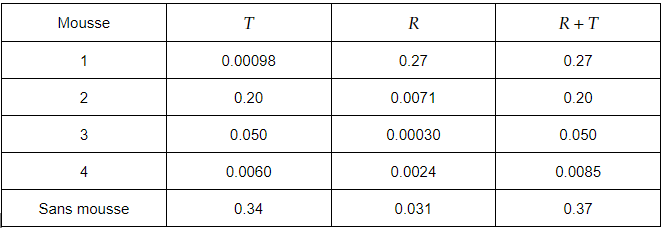
\includegraphics[scale=0.7]{img/tableau.png}
		\label{Stableau}
		\caption{Tableau récapitulatif de l'ensemble des coefficients $R, T, R+T$}
	\end{center}
\end{figure} 

Les coefficients sont cohérents avec la nature des mousses, les mousses dures ayant des coefficients de réflexion plus haut, mais un faible coefficient de transmission
alors que les mousses souples réfléchissent moins mais transmettent plus en comparaison. Nous mesurons un coefficient même sans écran car les ondes sont réfléchies sur le récepteur. 
 Cependant, nous remarquons un écart majeur à la théorie avec un coefficient $R+T$ loin de 1, ne rentrant 
clairement pas dans les incertitudes.
On suppose que les mousses absorbent une partie des ondes, mais nous ne savons pas si cela suffit à expliquer l'écart avec les valeurs théoriques.
Nous avons alors envisagé la possibilité d'une atténuation par l'air. Pour cela, nous avons suivi le protocole suivant. 

On mesure avec un récepteur collé à l'émetteur l'amplitude et l'on obtient $V = 1.7V$. On insère ensuite la mousse 2 et on mesure la réflexion et la transmission de l'onde.
Le récepteur en position de transmission reçoit $V=1.5V$ et le récepteur en position de réflexion reçoit $40mV$. Ce qui nous donne $T=0.78$ et $R=5.5\times 10^{-4}$, soit un $R+T \approx 0.78$. Les coefficients sont donc dépendants de la distance entre l'émetteur et l'écran. Cela peut être expliqué par le fait que l'émetteur envoie des ondes dans toutes les directions devant lui, les ondes ne sont pas focalisées. L'air peut aussi absorber une partie des ondes. 
 
Nous avons mis en évidence la présence d'un coefficient d'absorption dû à la présence
d'une mousse, et de l'atténuation de l'air, ce qui n'est pas pris en compte par le modèle.

\section{Conclusion}
Au cours de ce travail pratique, nous avons retrouvé la célérité d'une onde sonore dans des conditions standards de température et pression prédite par la théorie malgré des incertitudes considérables.
Cependant, la mesure par réflexion n'est pas concluante et n'entre pas en accord avec la théorie potentiellement par des variations de conditions d'expérimentations. Nous concluons également
que le modèle de réflexion/transmission n'est pas en accord avec nos expériences, et que ce modèle néglige la nature des matériaux pouvant absorber/amortir des ondes de façon non négligeable, et que l'atténuation
spatiale de l'onde n'est pas prise en compte. Pour améliorer le modèle il faudrait pouvoir proposer une loi décrivant l'amplitude de l'onde au cours de son déplacement dans un milieu pour pouvoir comparer le cas réel à la théorie.

\break
\section*{Annexes}
\subsection*{Démonstration de l'erreur sur l'approximation}
On rappelle que $d$ est la distance émetteur-écran, $e$ l'écart entre émetteur et récepteur et $h$ sera la distance réelle de l'aller.
\begin{align}
	h = \sqrt{d^2 + \frac{e^2}{4}} = d\sqrt{1+ \frac{e^2}{4d^2}}
\end{align}

La distance réelle est donc:
\begin{align}
	L = 2h = 2d\sqrt{1 + \frac{e^2}{4d^2}}
\end{align}

On pose que $e \ll d$ d'où:
\begin{align}
	L \approx 2d + \frac{1}{2} \frac{e^2}{4d^2}
\end{align}

Finalement, on peut déduire l'écart entre $c_{reel}$ et $c_{approx}$:
\begin{align}
	c_{reel} = \frac{L}{\Delta t} = \frac{2d + \frac{1}{2}\frac{e^2}{4d^2}}{\Delta t} = c_{approx} + \frac{1}{2}\frac{e^2}{4d^2 \times \Delta t}
\end{align}

Finalement, pour notre mesure où $d$ est la plus basse (donc l'approximation est plus susceptible d'être fausse), on obtient avec $d=30cm, e=2.3cm, \Delta t = 1.880ms$:
\begin{align}
	\delta c = c_{reel} - c_{approx} = \frac{1}{2}\frac{e^2}{4d^2 \times \Delta t} = 0.4
\end{align}
\end{document}